%
% File: chap05.tex
% Author: Nadeem Gul Rintu Daniel
% Description: Gives an Overview of the Geographic Coordinate System and the coordinate System which is implemented within the Floe Navigation System
%
\let\textcircled=\pgftextcircled
\chapter{System Design}
\label{chap:systemdesign}
\noindent
\initial{T}his section gives an overview of the Geographic Coordinate System. It will briefly introduce the concept of geographic coordinates and the Global Positioning System and how physical locations are mapped to coordinates on a $2$D plane. It also gives a detailed description of the custom coordinate system, which is derived from the Global Coordinate System, that is implemented as part of the Floe Navigation System.
%
\section{Floe Navigation App Architecture}
\label{sec:sec5_1}
\noindent
%
\textbf{\textcolor{red}{Add Description after name and screenshots are updated}}.The Floe Navigation App needs to calculate several important parameters at regular intervals to ensure that the coordinate system is calculated correctly and the points installed on the coordinate system are also placed properly. As shown in figure~\ref{fig:CH5AppArchitecture} the App uses several Services to ensure that the calculations are done correctly and at regular intervals.  
These Services run along with the App and are running as long as the App is running. However, when the App is used for the first time and the Coordinate System is not established yet, not all Services are running as some of these services can only work if there is a working coordinate system. Figure~\ref{fig:CH5AppStartup} shows the services, which are running before Grid Initial Configuration is completed.
\begin{figure}[!htb]
	\centering
	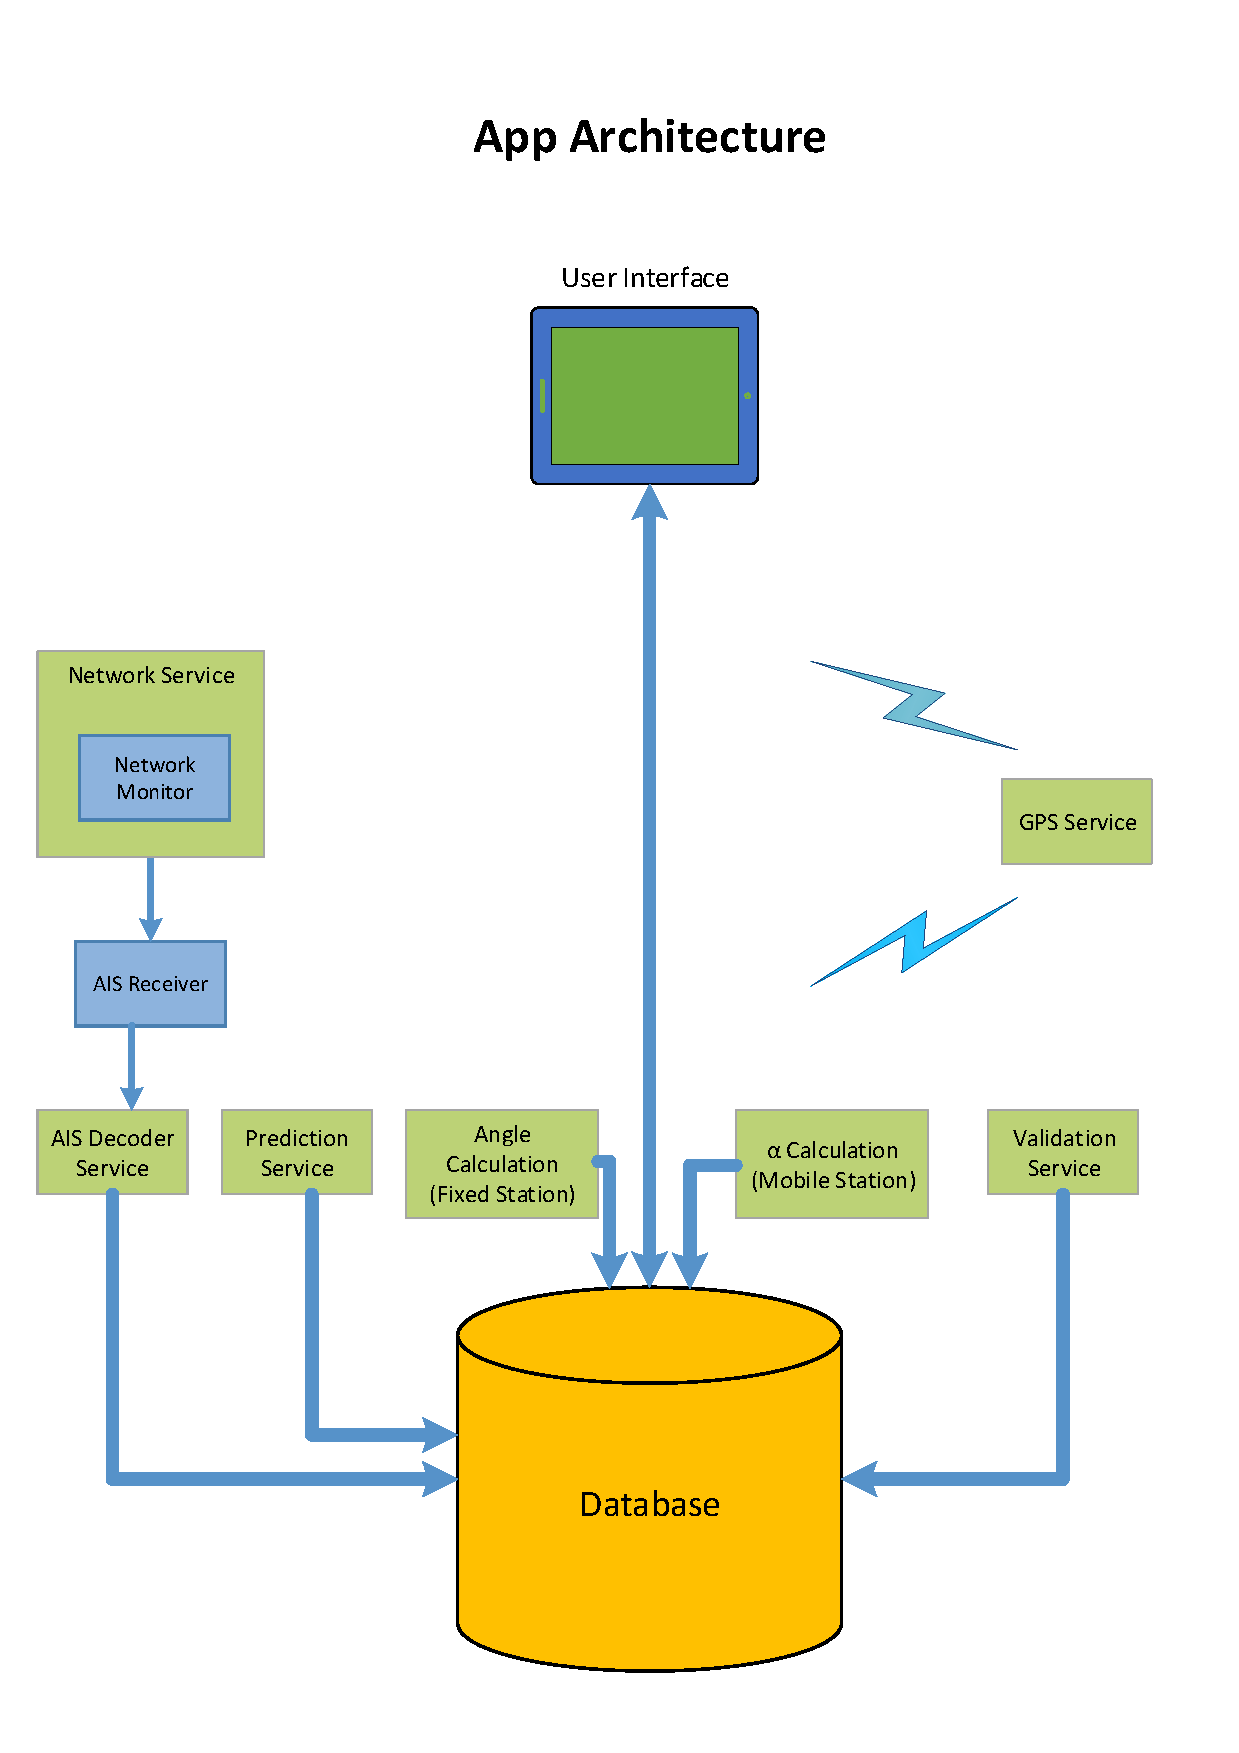
\includegraphics[width=.9\textwidth,height=.9\textheight]{fig05/App-Architecture}
	\mycaption[Floe Navigation App Architecture.]{Floe Navigation App Architecture.}
	\label{fig:CH5AppArchitecture}
\end{figure}
%
\newpage
\section{Services}
\label{sec:sec5_2}
\noindent
%
The Floe Navigation App needs to calculate several important parameters at regular intervals to ensure that the coordinate system is calculated correctly and the points installed on the coordinate system are also placed properly. As shown in figure~\ref{fig:CH5AppArchitecture} the App uses several Services to ensure that the calculations are done correctly and at regular intervals.
\newline
\noindent  
These Services run along with the App and are running as long as the App is running. However, when the App is used for the first time and the Coordinate System is not established yet, not all Services are running as some of these services can only work if there is a working coordinate system. Figure~\ref{fig:CH5AppStartup} shows the services, which are running before the initial configuration of the grid is completed.  
\begin{figure}[h]
	\centering
	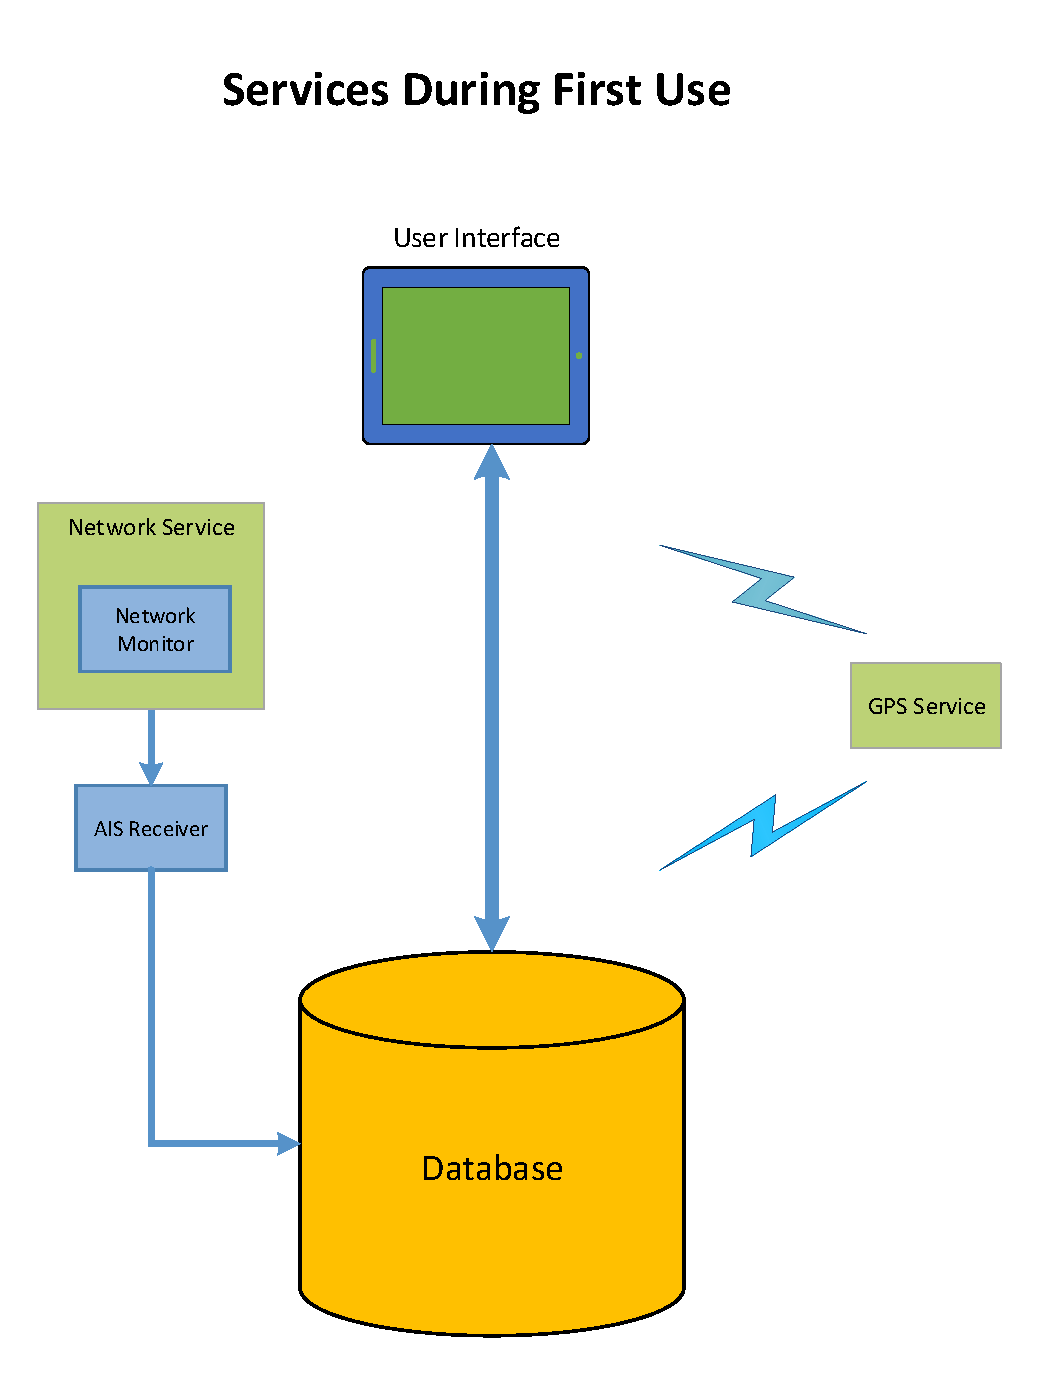
\includegraphics[width=0.7\textwidth,height=0.7\textheight]{fig05/AppStartup}
	\mycaption[Running Services during first use.]{Running Services during first use.}
	\label{fig:CH5AppStartup}
\end{figure}
%
\subsection{GPS Service}
\label{sec:sec5_2_1}
\noindent
%
GPS Service is responsible for reading the current location of the tablet and synchronizing time with the GPS Clock time. It runs in an individual thread and reads the location data from the GPS Provider within the tablet. The GPS provider does not use the Network Location Provider which uses internet and mobile network instead it uses satellite fix to determine the location of the device because of which the location fix may not work indoors.
\newline
\noindent
The GPS Service does not write the location to any particular location in the database instead it broadcasts the location data and other activities or services can read the location data from the broadcast. The GPS Service runs every \SI{30}{\second}.
%
\subsection{Network Service}
\label{sec:sec5_2_2}
\noindent
%
The Network Service ensures the connectivity of the App to the Wi-Fi network of an AIS transponder. It runs a Network Monitor thread which pings the AIS transponder every \SI{5}{\second}. The Network Monitor thread, in turn, starts another thread called AIS Message Receiver which then creates a Telnet Connection with the AIS transponder and starts receiving AIS Data using a buffered reader. 
\newline
\noindent
If the ping drops the already running AIS Message Receiver thread is terminated, and as soon as the ping is restored, the Network Monitor thread starts a new AIS Message Receiver thread so as to reestablish the Telnet Client. 
%
\subsection{AIS Decoding Service}
\label{sec:sec5_2_3}
\noindent
%
The AIS Decoding Service as its name suggests is responsible for decoding the incoming AIS packets. As explained previously the AIS Message Receiver thread creates a Telnet client which reads the incoming data using a buffered reader which can read the data line by line instead of byte by byte. As soon as a complete AIS packet is read, the AIS Message Receiver thread starts an AIS Decoding Service and passes it the packet. 
\newline
\noindent
The AIS Decoding Service then decodes the AIS Packet (for details on decoding check code documentation) and checks the MMSI of the incoming packet. If the MMSI is a Fixed Station it writes the data to the Fixed Station table otherwise it writes the data to the Mobile Station Table.
\newline
\noindent 
As the AIS Decoding Service is an Intent Service it runs in its own thread. However, as soon as its work is done and it has written the AIS data to the database it dies automatically.
\newline
\noindent
The AIS Decoding Service can only decode AIS packets of Type $1$, $2$, $3$, $5$, $18$ and $24$. For details on AIS Packet types and the information contained therein check \textbf{\textcolor{red}{Add Chapter Reference}}.
%
\subsection{Alpha Calculation Service}
\label{sec:sec5_2_4}
\noindent
%
This service calculates the position of each Mobile Station on the coordinate system. As explained in Chapter~\ref{chap:systemoverview}, any point on the coordinate system can be determined by the angle it makes with the x-Axis ($\alpha$) and the distance from the origin. As Mobile Stations can move on the Floe their angle $\alpha$ and distance need to be calculated at regular interval to ensure that the Mobile Stations are shown correctly on the Grid.
\newline
\noindent
The Alpha Calculation Service reads the mobile station data – such as latitude, longitude, speed over ground and course over ground – from the database and for each mobile station calculates the angle $\theta$ it makes with the Geographical Longitudinal Direction as shown in figure~\ref{fig:CH5AlphaCalculationService}. Then it calculates the difference between the angles $\theta$ and $\beta$ which gives $\alpha$. The Alpha Calculation Service calculates the distance from the origin using the Haversine formula (\textbf{\textcolor{red}{Citation}}).
\newline
\noindent 
The Alpha Calculation Service runs every \SI{10}{\second}. So, the position of each mobile station on the grid is updated every \SI{10}{\second} as well.
\begin{figure}[h]
	\centering
	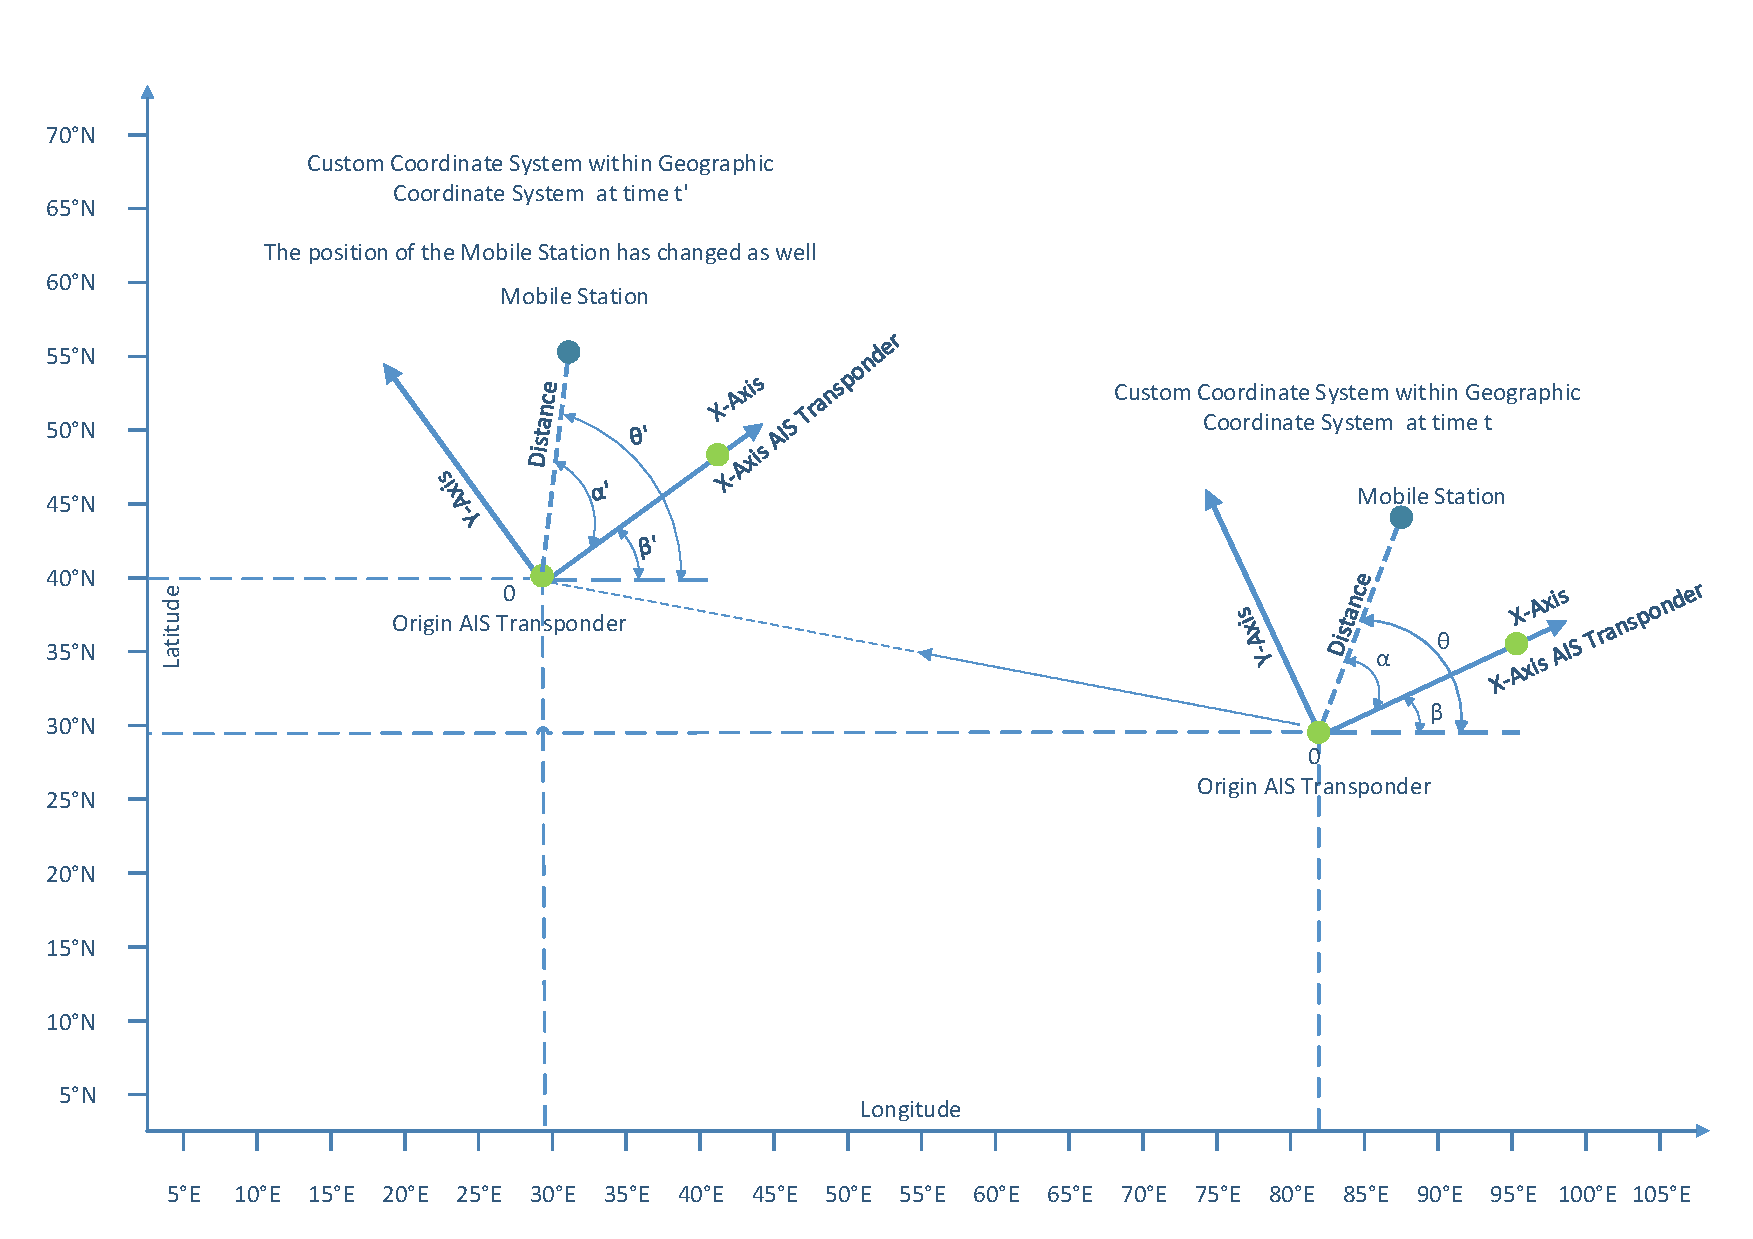
\includegraphics[height=0.45\textheight]{fig05/AlphaCalculationService}
	\mycaption[Mobile Stations within Coordinate System.]{Mobile Stations within Coordinate System.}
	\label{fig:CH5AlphaCalculationService}
\end{figure}
%
%
\subsection{Angle Calculation Service}
\label{sec:sec5_2_5}
\noindent
%
This Service is responsible for maintaining the coordinate system within the Geographical Coordinates. It updates the value of the angle $\beta$ which is used to create the coordinate system. The angle $\beta$ is calculated by using the fixed angle $\alpha$ and the distance from the origin of each Fixed Station. The new value for $\beta$ is the average of the $\beta$ calculated for each Fixed Station. This Service runs every \SI{10}{\second}.
%
\subsection{Prediction Service}
\label{sec:sec5_2_6}
\noindent
%
Most of the AIS transponders mounted on the Sea Ice are Class B AIS transponders which send their location data every \SI{3}{\minute}. However, for the Floe Navigation System, the update rate is much higher than \SI{3}{\minute} which means that the position of each Fixed Station on the Ice needs to be interpolated. Additionally, the predicted values can also help in detecting breakages in the Sea Ice by comparing the predicted values with the received values.
\newline
\noindent 
This Service predicts the position of each Fixed Station on the Ice at a much higher regular interval. It uses the Haversine formula (\textbf{\textcolor{red}{Citation}}) to calculate the position. For each station, it reads the current Latitude, Longitude, Speed Over Ground and Course Over Ground values and predicts what the Latitude and Longitude of that station will be in \SI{10}{\second} time. This Service also runs every \SI{10}{\second}.
%
\subsection{Validation Service}
\label{sec:sec5_2_7}
\noindent
%	
This Service is used to detect if a Fixed Station has broken off from the Floe. It calculates the difference in distance between the Predicted Coordinates (from the Prediction Service) and the Received Coordinates (from the AIS Decoding Service) and if the difference is more than a specified amount it marks the prediction as a wrong prediction. If several consecutive predictions go wrong within a specified interval of time for a given station that station is then removed from the Fixed Station table, is no longer used for calculations by other Services and is no longer visible on the Grid as a Fixed Station. 
In the special case when the origin station or the x-Axis marker station break off, the Floe Navigation App only removes their MMSI from the AIS Station list table so that the incoming data from these MMSI is not used for calculations. However, the Floe Navigation App keeps on showing a Fixed Station at the origin (with the MMSI $1000$) or x-Axis marker (with the MMSI $1001$) to preserve the grid visually. 
The difference in the distance which can mark a prediction wrong is defined by the \verb|ERROR_THRESHOLD| configuration parameter, and the time interval is defined by the \verb|PREDICTION_ACCURACY_THRESHOLD| configuration parameter. For details on the configuration parameters check \textbf{\textcolor{red}{Include Configuration Section}}.




